\begin{frame}
  \frametitle{课程介绍}
  \begin{itemize}
    \item Java是一门\textbf{非常重要}的课程,以后很多同学的毕业设计乃至工作都会使用到Java
    \item C/C++ 没学好,不代表你学不好Java!与前两者相比,这是一门相对“简单”的语言
    \item 数据结构没学好,不代表你学不好Java!本课程\textbf{偏向工程应用},很少涉及纯粹的算法
    \item 本课程包含绝大部分Java的基础知识,不包含Web相关内容
  \end{itemize}
\end{frame}

\begin{frame}
  \frametitle{课程要求}
  \begin{itemize}
    \item 实验课代码自己敲,不要复制粘贴!只会照着书或者PPT敲代码的,最后肯定学不好本课程!
    \item 作业算做实验课成绩。作业会有自动查重,不管谁抄谁,所有重复者作业(重复率大于70\%)一律0分!
    \item 本课程不设所谓的及格率下限!考试作弊者重修从严处理!大四清考按照正常出卷和判卷标准执行!
  \end{itemize}
  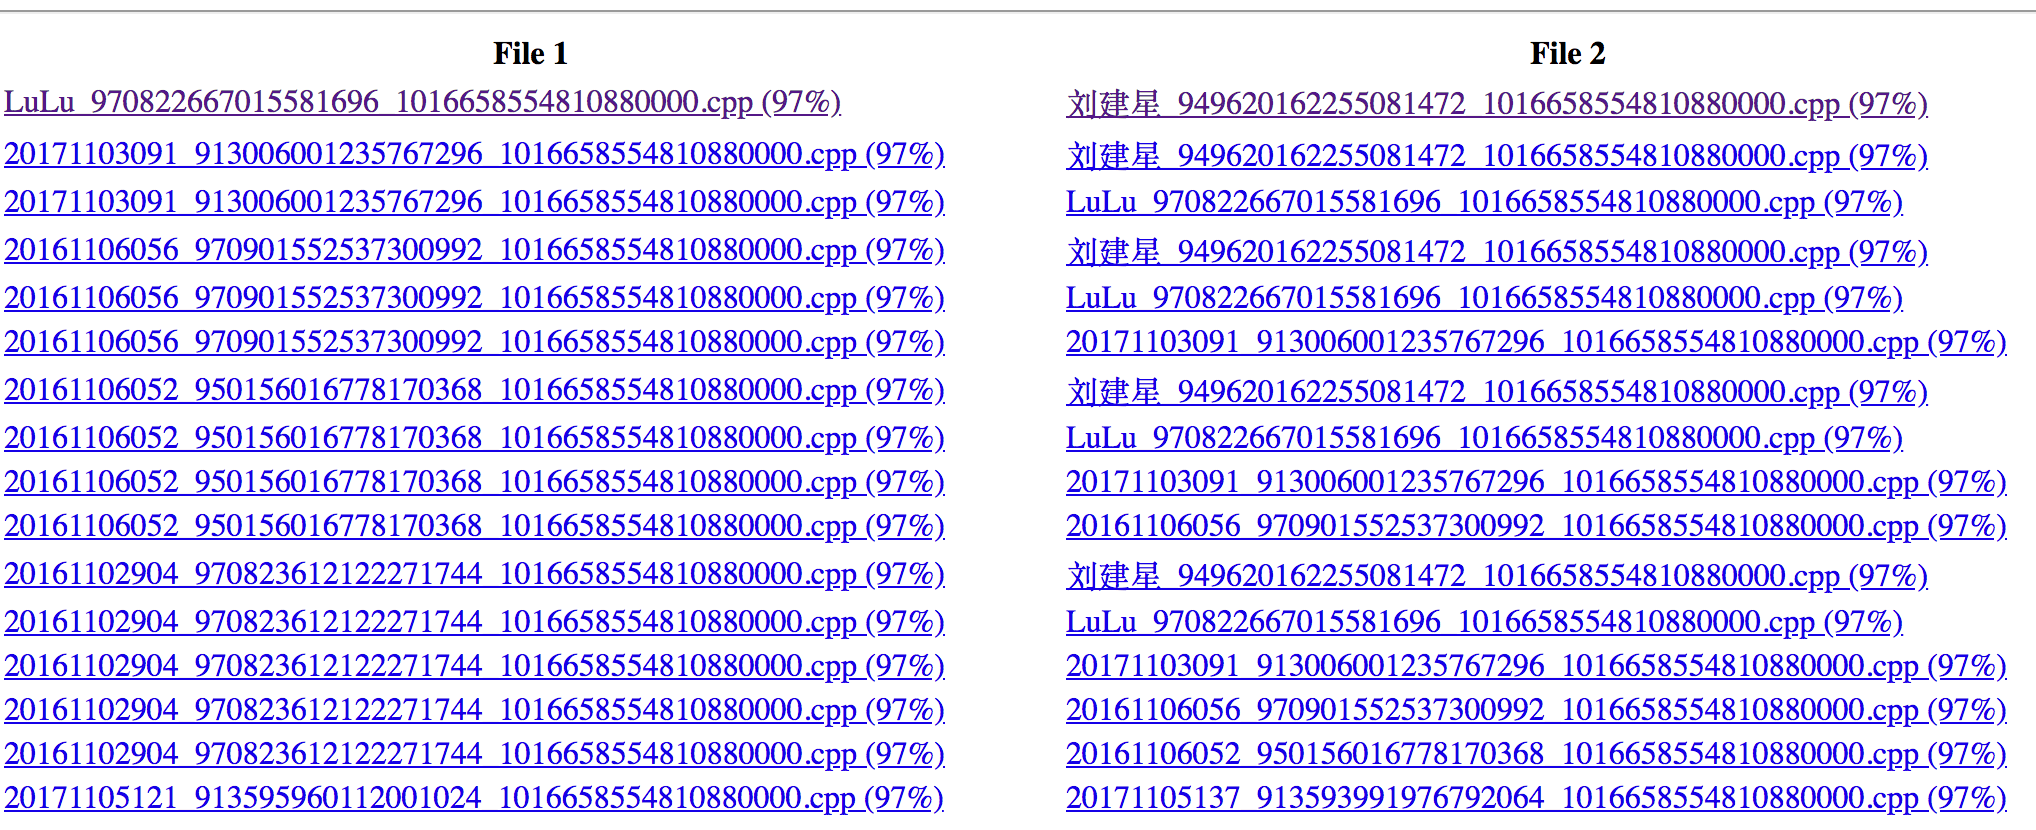
\includegraphics[width=\textwidth]{figures/moss}
\end{frame}


\begin{frame}
  \frametitle{Java语言的历史地位}
  \begin{enumerate}
    \item 第一代语言:打孔机,纯粹的机器语言,易于机器理解和执行。程序员需要掌握全部的硬件细节
    \item 第二代语言:汇编语言,比第一代语言更加容易编写,用抽象的符号表示指令、数据和寄存器,程序员需要掌握大量的硬件细节
    \item 第三代语言:高级语言,易于人类设计程序,对大部分硬件做了抽象
      \begin{itemize}
        \item 分类标准一:
          \begin{itemize}
            \item 面向过程的语言:C、Fortran、Pascal
            \item 不纯粹的面向对象的语言:C++
            \item 纯粹的面向对象的语言:Java
            \item 函数式语言:Lisp
          \end{itemize}
        \item 分类标准二:
          \begin{itemize}
            \item 编译型语言:C、C++、Java
            \item 解释型语言:Python、Javascript、Perl、PHP
          \end{itemize}
      \end{itemize}
  \end{enumerate}
  
  Java和Javascript是两种完全不同、毫无关系的语言!

\end{frame}

\begin{frame}
  \frametitle{Java语言的优点}
  \begin{itemize}
    \item “纯粹”的面向对象:不像C++那样包含过程化编程语言的要素
    \item 跨平台:通过Java虚拟机(JVM)实现了\textbf{平台无关性} ,一次编译,到处运行(write once, run everywhere)
    \item 开发效率高:易于编写、易于调试,易于团队合作,更加适合大型软件项目
    \item 健壮:吸收了C/C++的优点,同时去掉了其不太健壮的部分(如指针,内存的申请和释放),很大程度上缓解了“空指针”、“内存泄漏”等问题
    \item 易于学习:使得Java的使用人数多,且对Java程序员的要求较低
    \item 生态圈非常发达:可用软件工具包、中间件非常多,对于大多数类型的软件项目都不需要从头写起
  \end{itemize}
\end{frame}

\begin{frame}
  \frametitle{Java语言的缺点}
  \begin{itemize}
    \item 运行时效率较低(与C/C++相比):由“跨平台”的特点导致,编译后的Java程序并非直接运行在操作系统中,而是运行在JVM上    \item 语法冗繁,不够简明:由“易于学习”的特点导致,语言的表达能力不够,同样的一个语义,Java往往需要多行代码才能实现
    \item 对系统底层操控能力差:由“健壮”和“跨平台”的特点导致,不能使用JVM提供的功能和接口
  \end{itemize}
  
  \begin{block}{\textbf{设计语言时的考量}}
	\begin{itemize}
		\item “易于人类理解”还是“易于机器理解”:前者开发效率高,后者运行效率高
		\item “易于一般人使用”还是“易于聪明人使用”:前者表达力高,但是学习难度大;后者表达力低,但是学习难度低
		\item “更加底层”还是“更加抽象”:前者对系统操控能力大,后者不容易犯错(如空指针),更加安全
	\end{itemize}
  \end{block}
\end{frame}

\begin{frame}
  \frametitle{Java的应用领域}
  \begin{itemize}
    \item 适合的领域:
      \begin{itemize}
        \item Web服务器系统:如办公自动化、企业信息化、电子政务等
        \item 分布式应用:如Hadoop、HDFS等
        \item 数据密集型作业
        \item 有跨平台需求
        \item Android开发(采用Java语法和部分API)
      \end{itemize}
    \item 不适合的领域:
      \begin{itemize}
        \item 实时性要求高的系统:如军工、航控等
        \item 计算密集型作业:如科学计算、仿真模拟等
        \item 对性能要求苛刻的软件:如HTTP服务器、数据库等
        \item 底层设备驱动
      \end{itemize}
  \end{itemize}
    
  
\end{frame}

\begin{frame}
  \frametitle{Java程序运行机制}
  \begin{itemize}
    \item Java虚拟机(JVM,Java Virtual Machine)
    \item 垃圾收集机制
  \end{itemize}
  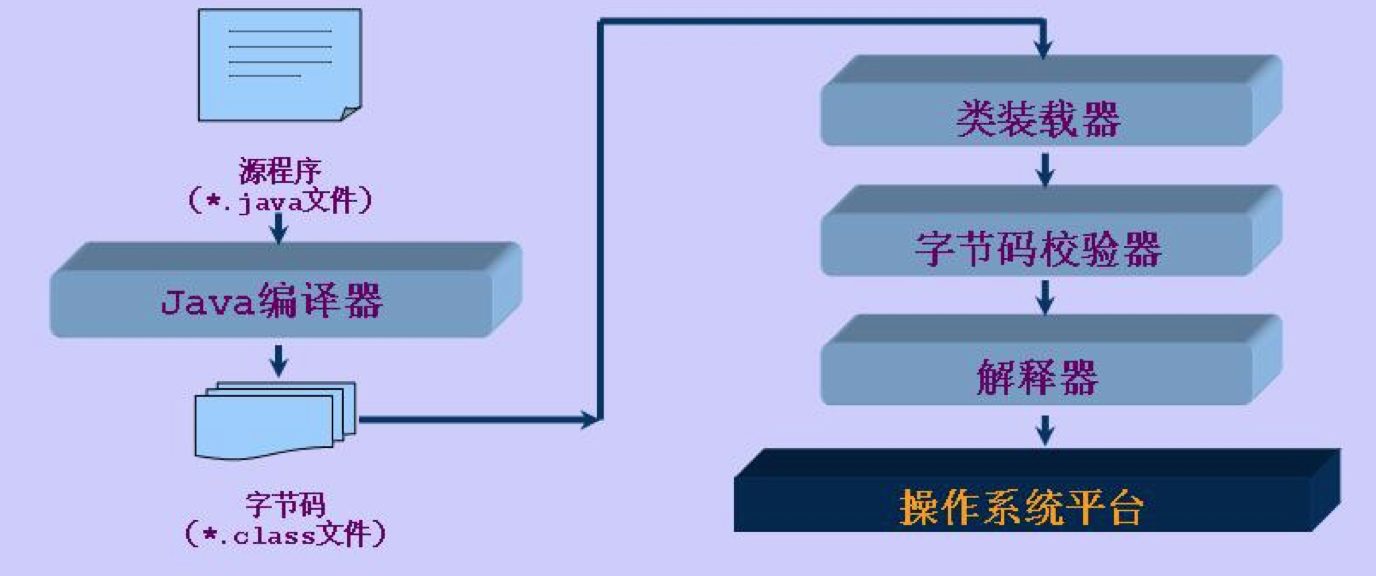
\includegraphics[width=\textwidth]{figures/java_workflow}
\end{frame}

\begin{frame}
  \frametitle{Java虚拟机(JVM)}
  \begin{itemize}
    \item Java源代码编译后形成的字节码无法被操作系统直接执行,只能被JVM执行
    \item JVM可以理解为一个以Java字节码为“机器指令”的虚拟CPU
    \item 不同的操作系统和平台有不同的JVM实现
    \item JVM位于操作系统之上,对其功能进行了封装,以此屏蔽了不同平台底层系统的差异性,实现“一次编译,到处运行”
  \end{itemize}
  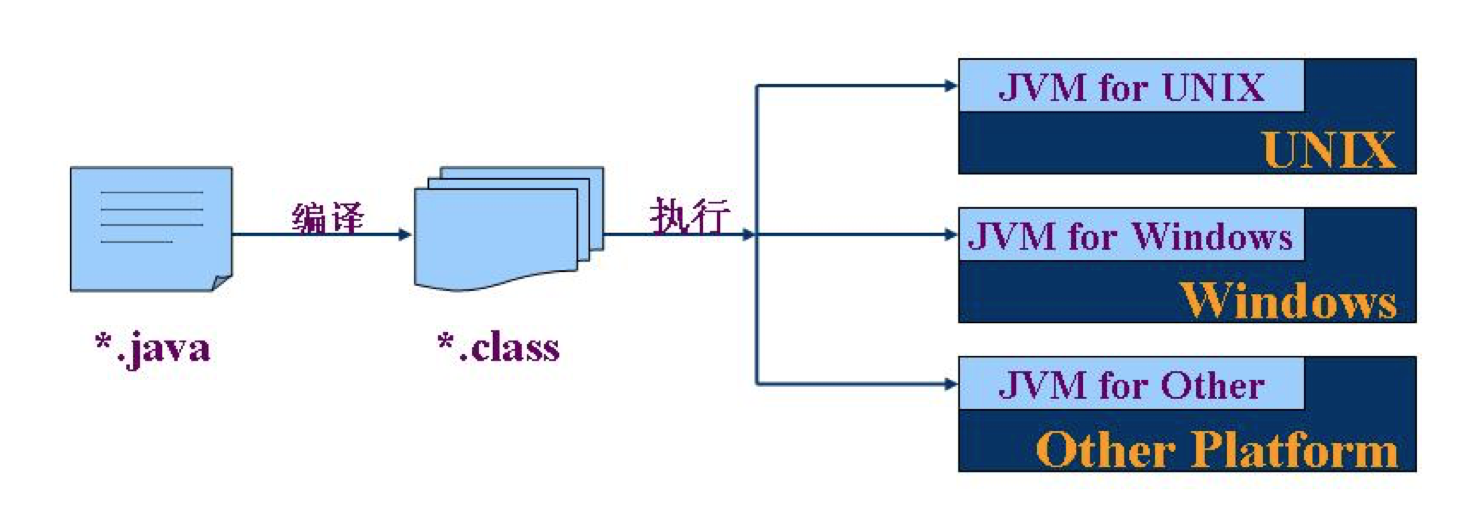
\includegraphics[width=\textwidth]{figures/jvm}

\end{frame}

\begin{frame}
  \frametitle{垃圾收集机制}
  \begin{itemize}
    \item 程序员无需也不能像C/C++中那样手动分配和回收内存(\texttt{malloc}、\texttt{free}等函数)
    \item 不再使用的内存空间会被JVM按照特定算法定期予以释放回收,此过程是JVM自动执行的,程序员无法精准的干预和控制
    \item Java的垃圾回收机制使程序员无需再承担内存管理的责任,有效降低了Java程序设计的复杂度和学习成本
  \end{itemize}
  \begin{block}{\textbf{JVM和垃圾收集带来的“负面影响”}}
    JVM在进行垃圾回收时是需要占用CPU资源的,此时整个JVM中运行的用户线程会停止工作,直到垃圾收集结束,这极大的影响了Java程序的实时性。对于C/C++这种手动管理内存的语言就不存在此问题,因为是程序员负责管理内存。
  \end{block}
\end{frame}

\begin{frame}
  \frametitle{Java发展史}
\begin{table}
\renewcommand\arraystretch{1.4}\arrayrulecolor{LightSteelBlue3}
\begin{tabular}{@{\,}r <{\hskip 2pt} !{\timeline} >{\raggedright\arraybackslash}p{9cm}}
1995 & JDK Beta\\
1996 & JDK 1.0	\\
1998 & J2SE 1.2	\\
2002 & J2SE 1.4	\\
2004 & J2SE 5.0,升级大版本号,直接从1.4升级为5.0\\
2006 & Java SE 6,将J2SE改名为Java SE(还包括Java EE,Java ME) \\
2009 & 年Oracle收购Sun,取得Java所有权\\
2014 & Java SE 8 (LTS,Long Term Support,长支持版本) \\
2018 & Java SE 10 \\
\end{tabular}
\end{table}
\end{frame}

\begin{frame}
  \frametitle{Java平台体系}
    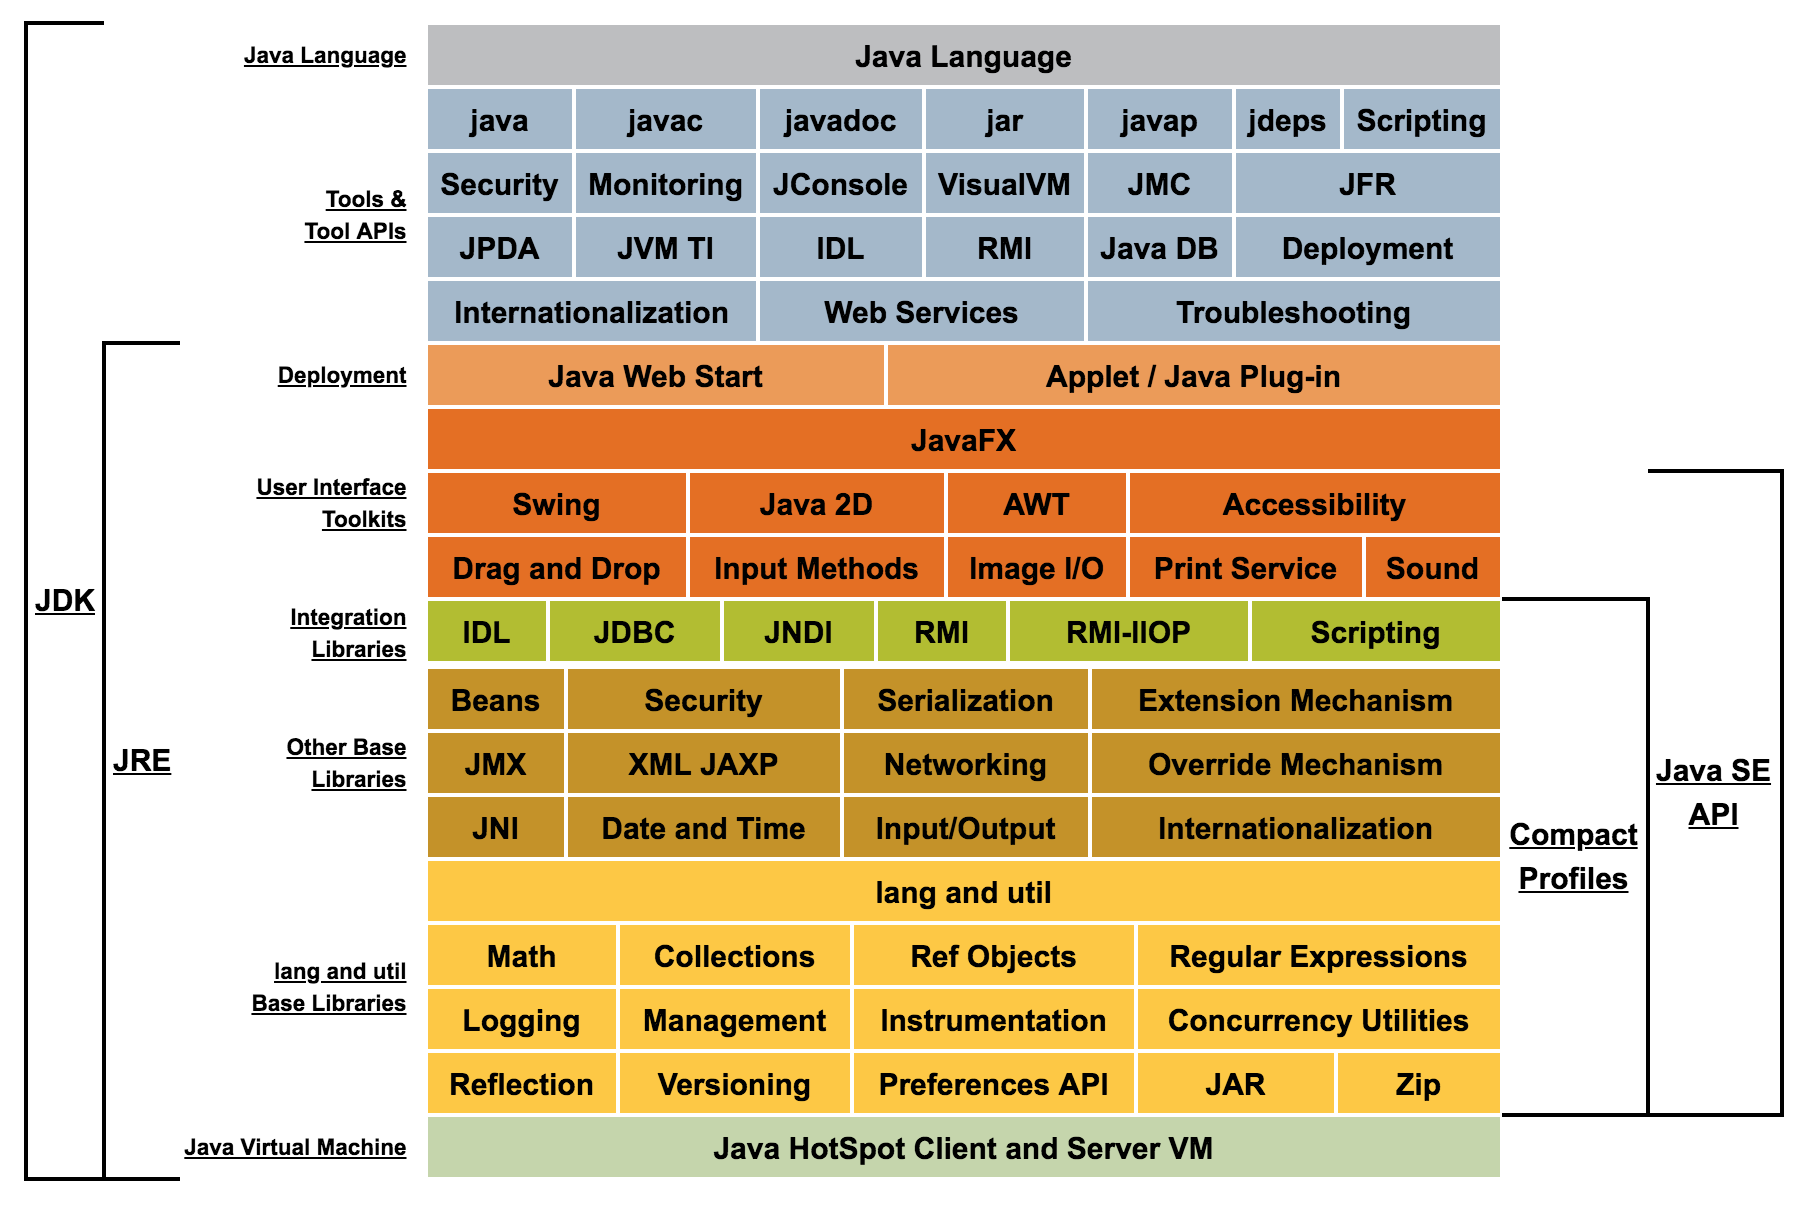
\includegraphics[width=\textwidth]{figures/java_conceptual_diagram}
\end{frame}

\begin{frame}
  \frametitle{Java平台体系中的概念要点}
  \begin{itemize}
    \item JDK和JRE:
      \begin{itemize}
        \item JRE:Java Runtime Environment,包含\textbf{用户运行编译后的Java程序的运行时环境}
        \item JDK:Java Development Kit,包含JRE以及\textbf{Java程序的开发工具包(编译、调试等)}。常用的JDK有官方的Oracle JDK、开源的Open JDK和IBM的J9(现开源为OpenJ9)
        \item 终端用户只需安装JRE即可,只有开发人员才需要安装JDK。JDK安装包较大
      \end{itemize}
    \item Java的版本
      \begin{itemize}
        \item Java ME: Java Micro Edition(逐渐被Android等所取代,用途越来越少,almost dead)
        \item Java SE:Java Standard Edition (主流版本)
        \item Java EE:Java Enterprise Edition(系统过于庞大复杂,应用场景也不多)
      \end{itemize}
  \end{itemize}
\end{frame}

